\section{Experiment}\label{sec:experiment}
In this section, we first evaluate the proposed training process on real dataset. Then we show the hardware experimental results. 

\subsection{Evaluation of Training}
We first evaluate the proposed training method with a software version implemented with Tensorflow. We use the VGG-11 model~\cite{simonyan2014very} on CIFAR-10 dataset for evaluation. The model consists of 8 convolution layers and 3 fully connected layers. We first test pruning the model after different normal training epochs. We train the model with floating point data and saves checkpoints after every 30 epochs. The saved checkpoints are pruned using the method in section~\ref{sec:training:prune}. The results are shown in Figure~\ref{fig:prune_exp}. The ratio of pruned weights does not vary greatly through the process of normal training. In general, most of the layers can be pruned to 40\% or less of the original size. This brings great potential of acceleration if hardware supports sparsity well.

\begin{figure}[tb]
  \centering
  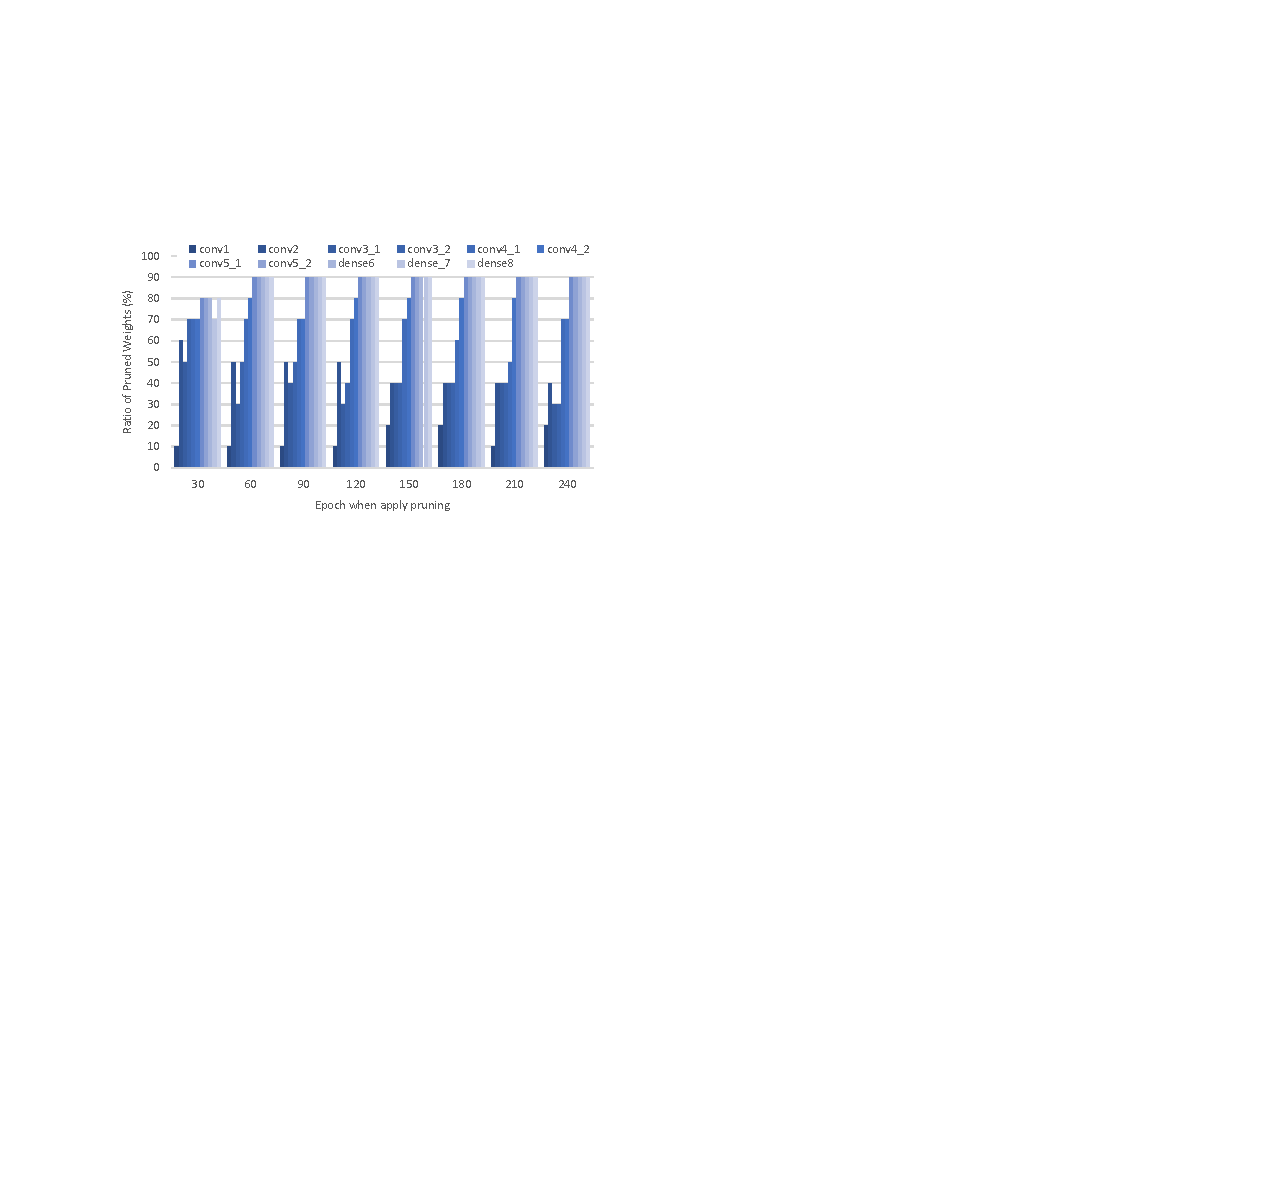
\includegraphics[width=1.0\columnwidth]{figures/pruning_exp.pdf}
  \caption{Ratio of pruned weights after different numbers of normal training epochs. }
  \label{fig:prune_exp}
\end{figure}

Then we test training the pruned models with different weight buffer sizes. We force the total training epochs to be 300. The model accuracy curves are shown in Figure~\ref{fig:fixed_train_exp}. When using 24-bit weight buffer, we see that training still works when gradients are quantized. But when to apply pruning and quantization matters. Starting as early as 30 epochs drops the final model accuracy from 90.62\% to 88.94\%. While starting as late as 240 epochs can even lead to worse result: the accuracy fluctuates around 87\%. Choose somewhere in the middle seems to bring good results but more experiments are needed to verify this conclusion. In this experiment, start quantization and pruning after only 60 epochs still brings 90.65\% accuracy at the end of training. When using 16-bit weight buffer, all the training stops after 120 epochs of training because the learning rate is too small while the bit-width is too short.

\begin{figure*}[tb]
  \centering
  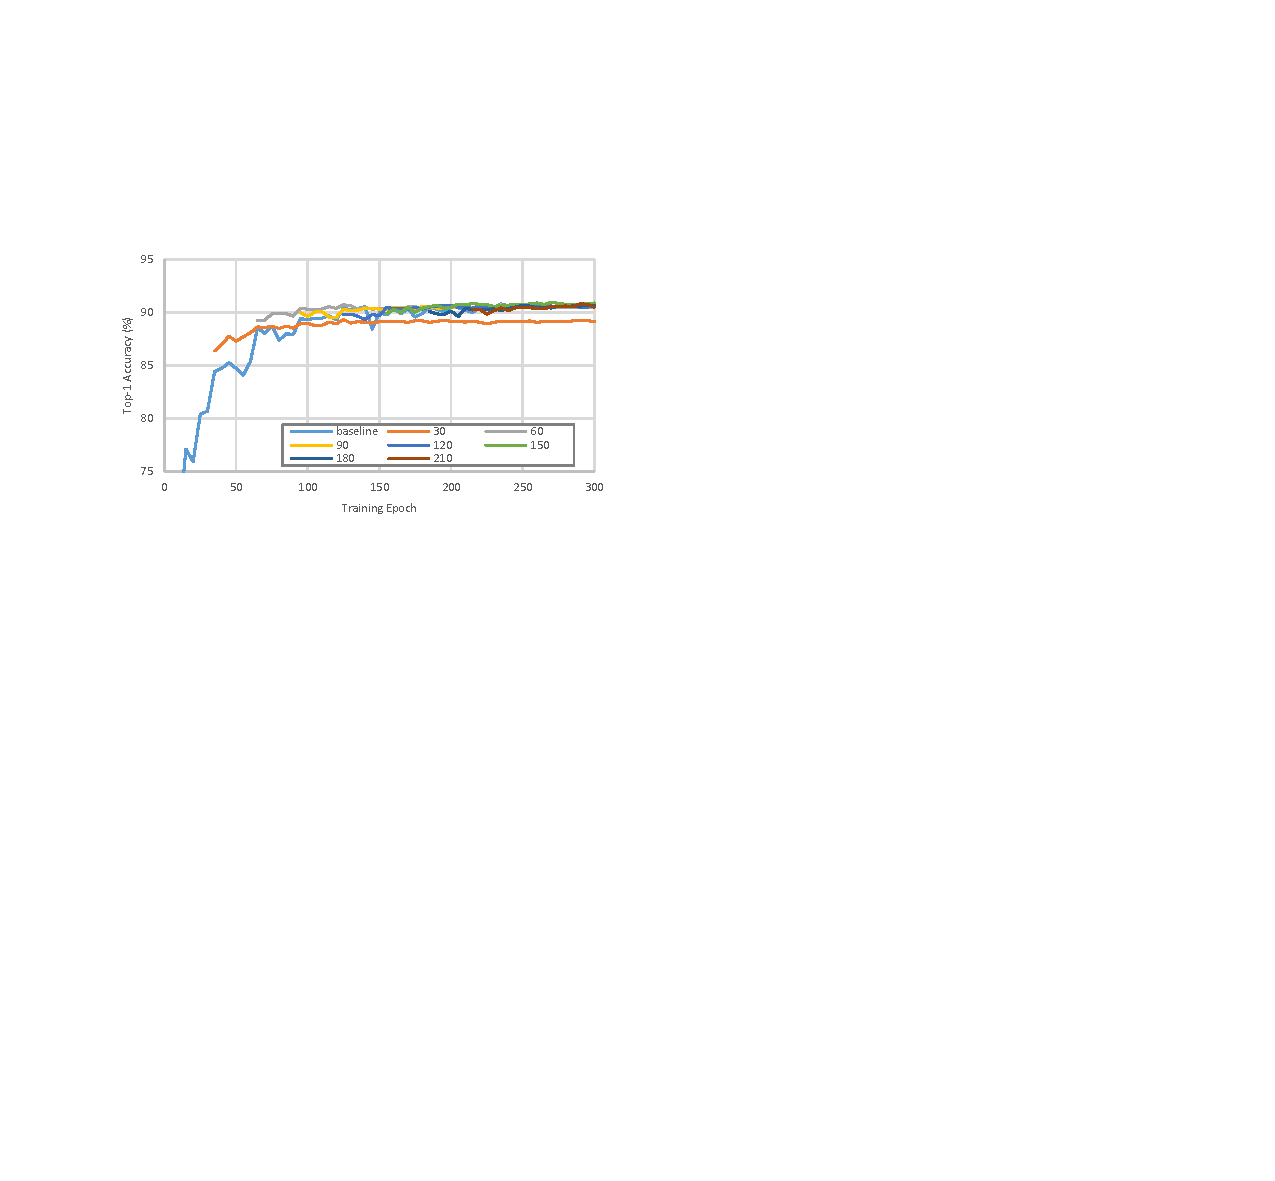
\includegraphics[width=2.0\columnwidth]{figures/fixed_train_exp.pdf}
  \caption{Accuracy curve of different training evaluation when quantization and pruning are applied at different stages. The number for each curve denotes the number of normal training epochs and baseline denotes a training without quantization and pruning. }
  \label{fig:fixed_train_exp}
\end{figure*}

\begin{table}[tb]
    \centering
    \caption{Prototype design resource utilization}
      \begin{tabular}{|c|c|c|c|c|}
      \hline
      Resource & LUT   & Reg   & Block RAM & DSP \\
      \hline
      Available & 663360 & 1326720 & 2160  & 5520 \\
      \hline
      Utilization & 199111 & 249122 & 1060   & 1030 \\
      \hline
      Ratio & 30\%  & 19\%  & 49\%  & 19\% \\
      \hline
      \end{tabular}
    \label{tab:util}
  \end{table}

\subsection{Effect of Workload Imbalance}\label{sec:exp:imb}

Before evaluating the hardware performance, we first analyze the theoretical performance loss brought by workload imbalance. As introduced in section~\ref{sec:hw_unroll}, unroll parameters are limited by loop dimension variety and sparsity. As we cannot group the PEs for fully connected layers, we only compare on the convolutional layers. The normalized speed on the convolutional layers of each configuration is shown in Table~\ref{tab:hw_util}.

\begin{table}[tb]
    \centering
    \caption{Comparison of PE utilization with different group sizes on a network}
      \begin{tabular}{|c|c|r|r|r|r|r|}
      \hline
      \multirow{2}[4]{*}{Layer} & Feature & Workload & \multicolumn{3}{c|}{Utilization} \\
  \cline{4-6}          & size & (MOP) & Single & 2x2 & Ideal\\
      \hline
      conv1 & $32\times 32$ & 3.54 & 80    & 88.5  & 100\\
      \hline
      conv2 & $16\times 16$ & 151 & 88.6  & 95.8  & 100\\
      \hline
      conv3\_1 & $8\times 8$   & 37.7 & 95.1  & 98.2  & 100\\
      \hline
      conv3\_2 & $8\times 8$   & 75.5 & 96.4  & 98.8  & 100\\
      \hline
      conv4\_1 & $4\times 4$   & 37.7 & 96.3  & 98.7  & 100\\
      \hline
      conv4\_2 & $4\times 4$   & 75.5 & 95.6  & 98.4  & 100\\
      \hline
      conv5\_1 & $2\times 2$   & 18.87 & 93.5  & 97.8  & 100\\
      \hline
      conv5\_2 & $2\times 2$   & 18.87 & 93.5  & 97.8  & 100\\
      \hline
      \multicolumn{3}{|c|}{Normalized Speed} & 0.928 & 0.974 & 1 \\
      \hline
      \end{tabular}
    \label{tab:hw_util}
  \end{table}

\begin{figure}[tb]
  \centering
  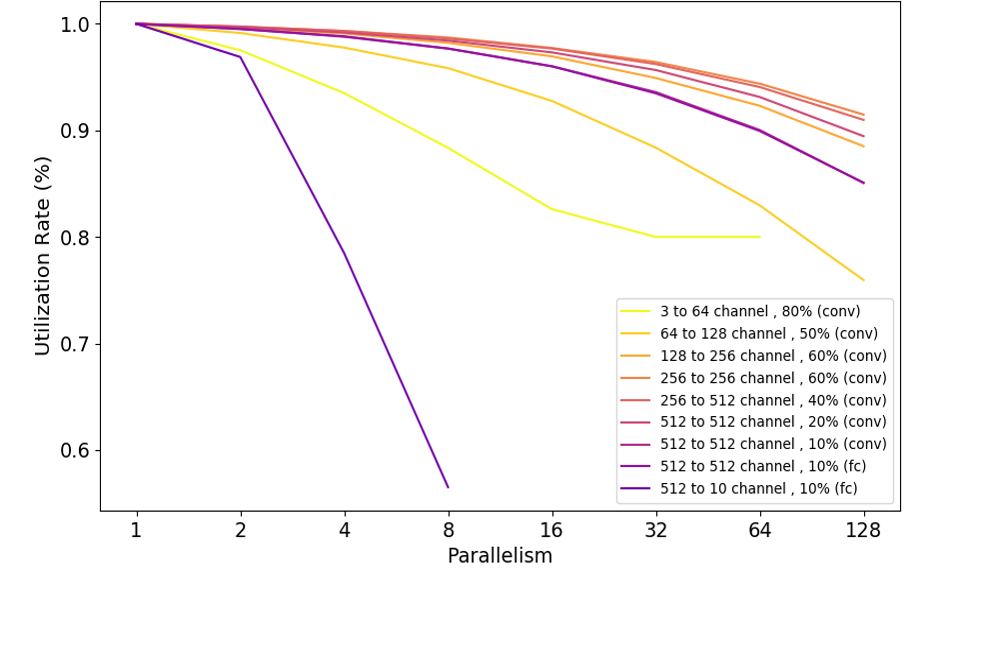
\includegraphics[width=1.0\columnwidth]{figures/util_real.png}
  \caption{Theoretical utilization ratio for each layer over the number of PEs.}
  \label{fig:util_real}
\end{figure}

Here, we see that using 32 PEs for this network will suffer from $7\%$ performance loss compared with the ideal case where no workload imbalance occurs. Group each 4 PEs together brings about $5\%$ performance increase. 


\subsection{Hardware Performance}
A prototype design is implemented on a Xilinx XCKU115 chip with 2 on-board DDR4 SDRAM. In this system, feature map, neuron and their gradients are all of 8-bit and stored in DDR0. Network weights, each of which includes 8-bit weight for computation and extra 16-bit buffer, are stored in DDR1. Corresponding index for sparse representation are stored in DDR0 using \{y[3:0], x[3:0]\} format. This means the the maximum weights block size can be $16\times 16$. The system operates at 200MHz. Each $2\times 2$ PEs are grouped together for CONV layers. We simulate the performance of each layer in each training step with the DDR model and controller from Xilinx IP. Detailed running time and performance are shown in Table~\ref{tab:layerperformance}.


\begin{table*}[tb]
    \centering
    %\footnotesize
    \caption{The performance of each layer. \textit{Comp.} indicates the complexity of each layer. \textit{Perf.} indicates the performance of running each layer on our hardware. \textit{Bound type} indicates the performance of each layer is bounded with bandwidth (B) or computation (C).}
    \begin{tabular}{c|c|cccc|cccc|cccc}  \hline
        &       & \multicolumn{4}{c|}{Forward Pass (FP)}  & \multicolumn{4}{c|}{Error Backpropagation (EB)} & \multicolumn{4}{c}{Weight Gradient (WG)} \\
  \cline{2-14}layer & Comp. & Time  & Perf. & bound & Utilize & Time  & Perf. & bound & Utilize & Time  & Perf. & bound & Utilize \\
        & (GOP) & (us)  & (GOP/s) & type  & rate  & (us)  & (GOP/s) & type  & rate  & (us)  & (GOP/s) & type  & rate \\
  \hline
  conv1 & 0.11  & 733   & 154.4  & B     & 27\%  & -     & -     & -     & -     & 4158  & 27.2  & B     & 5\% \\
  conv2 & 1.21  & 1487  & 812.2  & C     & 95\%  & 1487  & 812.5  & C     & 95\%  & 2804  & 430.8  & B     & 50\% \\
  conv3\_1 & 1.21  & 1696  & 712.4  & C     & 97\%  & 1694  & 713.0  & C     & 97\%  & 2477  & 487.7  & B     & 67\% \\
  conv3\_2 & 2.42  & 2877  & 839.7  & C     & 98\%  & 2876  & 840.1  & C     & 98\%  & 4398  & 549.3  & B     & 64\% \\
  conv4\_1 & 1.21  & 1217  & 992.3  & C     & 97\%  & 1217  & 992.9  & C     & 97\%  & 2686  & 449.8  & B     & 44\% \\
  conv4\_2 & 2.42  & 1457  & 1658.4  & C     & 97\%  & 1456  & 1659.2  & C     & 97\%  & 3933  & 614.2  & B     & 36\% \\
  conv5\_1 & 0.60  & 366   & 1651.7  & B     & 32\%  & 358   & 1687.7  & B     & 33\%  & 915   & 659.8  & B     & 13\% \\
  conv5\_2 & 0.60  & 365   & 1652.7  & B     & 32\%  & 358   & 1688.7  & B     & 33\%  & 915   & 660.0  & B     & 13\% \\
  dense6 & 0.02  & 329   & 51.0  & B     & 1\%   & 328   & 51.1  & B     & 1\%   & 717   & 23.4  & B     & 0.5\% \\
  dense7 & 0.02  & 329   & 51.0  & B     & 1\%   & 328   & 51.1  & B     & 1\%   & 717   & 23.4  & B     & 0.5\% \\
  dense8 & 0.003  & 75    & 4.4   & B     & 0.1\% & 74    & 4.4   & B     & 0.1\% & 272   & 1.2   & B     & 0.02\% \\
  \hline
  total & 9.81  & 10931  & 897.5  & -     & -     & 10988  & 892.8  & -     & -     & 23993  & 408.9  & -     & - \\
  \hline
  \end{tabular}%
    \label{tab:layerperformance}%
  \end{table*}%

% Table generated by Excel2LaTeX from sheet 'Sheet1'
% Table generated by Excel2LaTeX from sheet 'Sheet1'
\begin{table*}[htbp]
    \centering
    \caption{Performance comparison between the proposed accelerator and existing CNN inference/training accelerators and GPU}
      \begin{tabular}{|l|c|c|c|c|c|c|c|c|c|c|}
      \hline
      \multirow{2}[4]{*}{Platform} & \cite{guo2017angel} & \cite{ma2017optimizing} & \cite{han2017ese} & \multicolumn{2}{c|}{\cite{zhao2016f}} & \cite{liu2017fpga} & \cite{geng2018fpdeep} & \multicolumn{2}{c|}{Proposed} & Titan X \\
  \cline{2-10}          & \multicolumn{1}{l|}{XC7Z020} & GX1150 & KU060 & \multicolumn{2}{c|}{Maxeler MPC-X} & ZU19EG & VC709 & \multicolumn{2}{c|}{KCU1500} &  GM200 \\
      \hline
      Function & Inference & Inference & Inference & Inference & Training & Training & Training & Inference & Training & Training \\
      \hline
      Quantization & fixed 8 & fixed 8/16 & fixed 12 & float 32 & float 32 & float 32 & fixed 16 & fixed 8 & fixed 8/24 & float32 \\
      \hline
      Sparsity & No    & No    & Yes   & No    & No    & No    & No    & Yes   & Yes   & No \\
      \hline
      Performance & \multirow{2}[2]{*}{84.3} & \multirow{2}[2]{*}{645.25} & \multirow{2}[2]{*}{2516} & \multirow{2}[2]{*}{62.06} & \multirow{2}[2]{*}{7.01} & \multirow{2}[2]{*}{86.12} & 1022  & \multirow{2}[2]{*}{897.5} & \multirow{2}[2]{*}{641.1} & \multirow{2}[2]{*}{1252} \\
      (GOP/s) &       &       &       &       &       &       & (Per FPGA) &       &       &  \\
      \hline
      Power (W) & 3.5   & 21.2  & 41    & N.A.  & 27.3  & 14.2  & 32    & \multicolumn{2}{c|}{26.8} & 150 \\
      \hline
      Energy Eff. & \multirow{2}[2]{*}{24.1} & \multirow{2}[2]{*}{30.43} & \multirow{2}[2]{*}{61.4} & \multirow{2}[2]{*}{N.A.} & \multirow{2}[2]{*}{0.27} & \multirow{2}[2]{*}{6.05} & \multirow{2}[2]{*}{31.97} & \multirow{2}[2]{*}{33.61} & \multirow{2}[2]{*}{24.01} & \multirow{2}[2]{*}{8.4} \\
      (GOP/s/W) &       &       &       &       &       &       &       &       &       &  \\
      \hline
      \end{tabular}%
    \label{tab:perf_compare}%
\end{table*}%

The peak performance of the hardware is $250MHz \times 1024DSP \times 2 = 500GOP/s$. For FF and NG steps, the proposed hardware achieves 900GOP/s overall performance which achieves at least $1.8\times$ speedup over a dense accelerator with the same peak performance. From the bound type column, we see that most of the CONV layers with heavy workload are computation bounded. This shows that the proposed accelerator can handle large network well.

Besides that, those layers which are bandwidth bounded gives insights to hardware design methods. The first layer suffers from the bandwidth problem because the channel number for this layer is small. We only cut $3\times 8$ block for this layer. A small block size increases the ratio between the necessary feature maps and the necessary convolution kernels. Compared with the workload imbalance result in \ref{sec:exp:imb}, we see that small layers suffer more on bandwidth rather than workload imbalance. Besides reducing the number PEs, increase the buffer size in PEs can help further explore the data locality of 2-d convolution and improves performance. 

The last few layers also suffers greatly from a limited bandwidth. On the one hand, FC layers and convolution layers with small feature maps are of high bandwidth cost for network parameters. On the other hand, split the parameters into small blocks decreases the memory access efficiency. When upgrading the weights of each layer, the weight buffer consumes more bandwidth and causes the performance loss. Reduce the weight buffer size should also be a future research topic. 

A performance and energy efficiency comparison is with state-of-the-art neural network inference/training accelerators and GPU training result is shown in Table~\ref{tab:perf_compare}. The GPU used for comparison is GTX Titan X GM200. Although GPU achieves about 2x speed compared with FPGA, the FPGA part only consumes 1/5 power compared with GPU and achieves 3x energy efficiency. The proposed accelerator achieves much higher energy efficiency compared with the designs~\cite{liu2017fpga, zhao2016f} using floating point data.

The performance of the proposed design is still not as good as FPDeep~\cite{geng2018fpdeep}. This may be caused by two reasons. The first reason is that FPDeep use plain 16-bit fixed point data for training. The proposed design is mainly limited by memory system because of the large weight buffer used for accumulation. FPDeep also stores all the weights of convolution layers on-chip by using multiple FPGAs. The second reason is that FPDeep designs computation kernels for each layer independently, which leads to high utilization ratio. This shows that scaling down FPDeep is hard. We will also explore ways to scale up the proposed design in the future.









